One of the major difficulties with studying nucleation and crystal growth with computer simulations is the temporal limitations of molecular dynamics and the lack of dynamic information in Monte Carlo simulations. Metadynamics has been proposed as a alternative computer simulation method that overcomes the deficiencies of molecular dynamics and Monte Carlo simulations.  Metadynamics is based on the energy landscape framework, which has had great success in describing microscopic behavior in a range of materials.  In this chapter, we will first present the energy landscape framework and the multitude of information contained in the landscape.  Then, we will present our improved metadynamics method for directly sampling the energy landscape.  Lastly, we will discuss the implementation of the method into GROMACS, and how to analyze the metadynamics simulation output.

\section{Energy Landscape}
The potential energy landscape formulation is a framework developed originally by Goldstein in 1969 \cite{Goldstein1969} for the study of viscous liquids and the glass transition.  This framework has been extended by many since the original formulation to explain slow phenomena and out of equilibrium behavior including protein folding, supercooled liquids, phase behavior, and more \cite{Shell2003}\cite{Middleton2001}\cite{Angell1997}\cite{Debenedetti2001}.  A two dimensional schematic of an potential energy landscape is shown in Figure \ref{energy_landscape} \cite{Debenedetti2001}.

\begin{figure}[h]
	\centering
	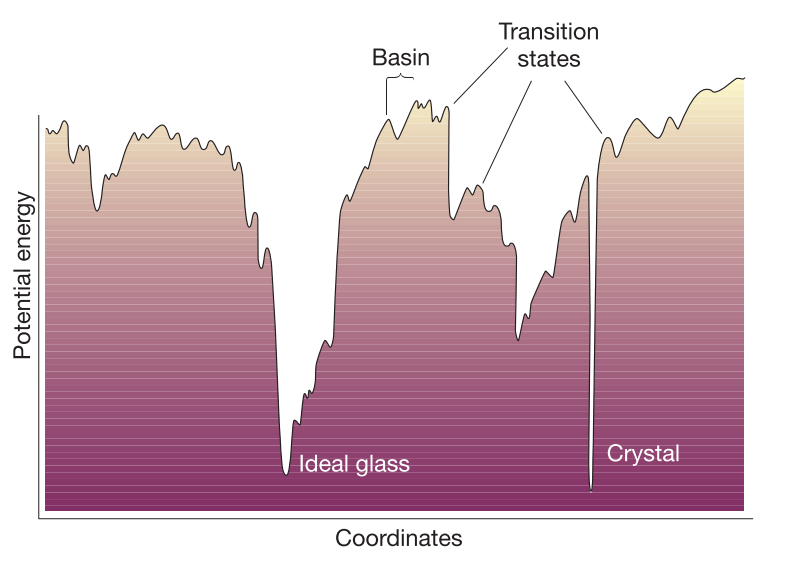
\includegraphics[width = .5\textwidth]{./Figures/MTD/Energy_landscape.png}
	\caption[A schematic plot of the potential energy landscape in 2-D (potential energy versus 1 configurational coordinate).  The true potential energy landscape is multi-dimensional depending on the number of configurational coordinates; the dimensionality can range from 1 to 3N if all atoms coordinates are used.]{A schematic plot of the potential energy landscape in 2-D (potential energy versus 1 configurational coordinate).  The true potential energy landscape is multi-dimensional depending on the number of configurational coordinates; the dimensionality can range from 1 to 3N if all atoms coordinates are used. \cite{Debenedetti2001}}
	\label{energy_landscape}
\end{figure}

Figure \ref{energy_landscape} shows a schematic of the potential energy landscape and the diverse features typical of the potential energy landscape \cite{Debenedetti2001}.  It is important to note that this schematic drawing is reduced to two dimensions (the potential energy and a single configurational coordinates), a typical potential energy landscape is hyper dimensional ranging from one dimension to 3N dimensions, where N is the number of atoms in the system.  Examples of configurational coordinates are the bond angles in protein (several configurational coordinates) \cite{Wales2012}, the system bond orientational order parameter for ordered structures (one to a couple of configurational coordinates) \cite{Quigley2008}, and the XYZ position coordinates of each atom (3N configurational coordinates) \cite{Kushima2009, Kushima2009a}. The more degrees of freedom the higher the dimensionality, and the more complex the potential energy landscape becomes.  As a result of the hyper dimensionality, methods to calculate the landscape are still limited.  Generally, the landscape is used as a theoretical framework to explain atomic scale phenomena, both structural and dynamical.

While the potential energy landscape is typically higher dimensional than Figure \ref{energy_landscape}, much can be learned from the 2-D dimensional potential energy landscape.  Figure \ref{energy_landscape} shows the potential energy landscape is rich in energy minimums, with variable potential energy.  The probability of occupying a particular potential energy minimum with energy $G$ is proportional to $\exp(\frac{-G}{k_BT})$.  Thus, at high temperatures, the system can occupy both high energy and low energy minimums with high likelihood \cite{Royall2015}.  As the temperature decreases the chance of occupying high energy (disordered states) becomes less likely, and the system tends to occupy the lower energy minimums (ordered states) \cite{Royall2015}.  Because the potential energy landscape is richer in high energy states than low energy states, the occupation of lower energy states with decreasing temperature leads to a decrease in configuration entropy \cite{Royall2015}.  At sufficiently low temperatures, any medium to high energy basins become inaccessible leading to dynamic arrest, and the formation of  metastable materials \cite{Royall2015}.

In this way, the potential energy landscape is used to explain the structural state of a system, the minimums represent different structural states \cite{Debenedetti2001}.  In order for the system to evolve structurally, the system must overcome energy barriers separating the minimums  \cite{Debenedetti2001}.  This dynamical process is related to the height of the energy barrier and the temperature of the system similar to the occupation probability of different energy minimum \cite{Debenedetti2001}.  The larger the barrier the less likely the system will relax from one minimum to another  \cite{Debenedetti2001}.  Further the likelihood of crossing a barrier is related to the thermal energy in the system.  In this way, as a system is cooled, the system can become stuck in deep energy minimums that are not the lowest energy state.  Because the energy barriers are too high to overcome the system is trapped in this metastable state, or glass state.  

In MD simulations, we can study many equilibrium features of the potential energy landscape.  In the crystal state, MD will capture the vibrations in the deep crystal minimum, or phonons \cite{Debenedetti2001}.  In the disordered supercooled liquid or glassy state, MD will capture the relaxation times as the system evolves over energy barriers between energy minimum of similar potential energy \cite{Debenedetti2001}.  However, as Figure \ref{energy_landscape} shows, the energy barrier between the glassy basin and the crystal basin is significantly large, such that the probability of the system to evolve from the ideal glass state to the crystal state is improbable, and likely to occur over only long timescales inaccessible by MD.  Similarly, MC is used to sample the energy minimums of the potential energy landscape with likelihood $\exp(-\frac{G}{k_BT})$.  However, MC does not provide energy barrier information (dynamical information), which is essential to understanding the temporal element of a kinetic process, such as nucleation.  For this reason, in order to study kinetic events at the atomic scale, advanced sampling methods capably of sampling macroscopically long time behavior is required.  Further, the method needs to sample the energy barrier height and the energy minimums separating the two deep basins.

\section{Metadynamics Method}
Currently, the prevalent method for simulating atomic scale systems with computers is with molecular dynamics and Monte Carlo simulations.  Molecular dynamics provides a great deal of information about the structure and dynamics of a system.  However, molecular dynamics is heavily limited by its accessible timescale \cite{Melorose2015}.  In order to accurately integrate Newton's equations (the foundation of molecular dynamics) a time step on the scale of molecular vibrations is required, typically on the scale of femtoseconds \cite{Melorose2015}.  As a result, molecular dynamics at best can access time scales of up to microseconds.  While microseconds can be sufficient for equilibrium studies, transient events such as nucleation requires orders of magnitude larger in timescale.  Recent work on metadynamics methods show promise for overcoming this temporal restraint while simultaneously providing basin and barrier information.  Metadynamics use a potential bias to drive the system from energy minimums, preventing arrest in anyone minimum \cite{Melorose2015}.  The method overcomes large barriers allowing for direct sampling of a larger region of the potential energy landscape \cite{Melorose2015}.

Metadynamics simulations begin with a arbitrary configuration, typically this will be a metastable configuration, as shown in Figure \ref{landscape filling}A.  This configuration is represented by $\mathbf{r}_{\min}^\alpha$, where $\alpha$ represents the number of penalties applied, in this case 0 \cite{Kushima2009, Kushima2009a}.  The system configuration during the simulation is represented by $\mathbf{r}$.  From this point we add a penalty function $\phi$, which can take any shape, but we choose to use Gaussian functions
\begin{equation}
\phi(\mathbf{r},\mathbf{r}_{\min}^\alpha) = H\exp\left(\frac{-\left(\mathbf{r} - \mathbf{r}_{\min}^\alpha\right)^2}{2\sigma^2}\right)
\end{equation}
where $H$ is the height of the penalty function, and $\sigma$ is the width of the penalty function \cite{Kushima2009, Kushima2009a}.  Appropriate choices for the penalty function variables $H$ and $\sigma$ are discussed in the following sections.  We choose to use a Gaussian function because it is symmetric in all directions and quickly decays, thus it is local on the landscape \cite{Kushima2009, Kushima2009a}.  If we choose a function that does not locally decay, the function may also affect surrounding basins and saddle points.  This added potential results in a force on each atom of
\begin{equation}
	\mathbf{F}^\alpha(\mathbf{r},\mathbf{r}_{\min}^\alpha) = -\nabla \phi(\mathbf{r},\mathbf{r}_{\min}^\alpha)
\end{equation}
\begin{equation}
	\mathbf{F}^\alpha(\mathbf{r},\mathbf{r}_{\min}^\alpha) = \frac{H}{\sigma^2}\left(\mathbf{r} - \mathbf{r}_{\min}^\alpha\right)\exp\left(\frac{-\left(\mathbf{r} - \mathbf{r}_{\min}^\alpha\right)^2}{2\sigma^2}\right)
\end{equation}
This force is added to the force created by the pair potential of the system.  As more penalties are applied the total potential and force on the system becomes
\begin{equation}
\begin{split}
	\Phi(\mathbf{r}) &= U(\mathbf{r}) + \sum_{\alpha}\phi(\mathbf{r},\mathbf{r}_{\min}^\alpha) \\
	\mathbf{F}(\mathbf{r}) &= \mathbf{F}_{pp}(\mathbf{r}) + \sum_{\alpha}\mathbf{F}^\alpha(\mathbf{r},\mathbf{r}_{\min}^\alpha)
\end{split}
\end{equation}
where $\mathbf{F}_{pp}(\mathbf{r})$ is the force generated from the pair potential, $\Phi(\mathbf{r})$ is the potential energy of the system post penalty function, $U(\mathbf{r})$ is the potential energy of the system without the penalty functions, and $\mathbf{F}(\mathbf{r})$ is the force applied to the system with the penalties applied.  Again, $\mathbf{r}^\alpha_{min}$ represents the different locations that penalties have been applied, and $\alpha$ is the number of penalties applied \cite{Kushima2009, Kushima2009a}.  By applying these penalty functions the potential energy landscape has now been changed, as shown by Figure \ref{landscape filling}B.  The figure shows the added penalty energy in blue, thus the landscape has changed from figure panel A to B.  We then apply Newton's steepest descent algorithm to search for the most local minimum on the new landscape \cite{Kushima2009, Kushima2009a}.  
\begin{equation}
\begin{split}
	\mathbf{r}_{i+1} &= \mathbf{r}_{i} - \delta\nabla\Phi(\mathbf{r}) \\
					 &= \mathbf{r}_{i} + \delta\mathbf{F}(\mathbf{r})
\end{split}
\end{equation}
where $i$ is the iteration of Newton's steepest descent, and $\delta$ is the step size of each iteration in units of distance.  The force in the previous equation is normalized by force of the atom with the maximum force, and is as a result unitless.  $\delta$ determines the stability of the algorithm.  Once Newton's steepest descent has converged, the configuration is considered to be in a new local minimum of $\Phi$-space, we denote this configuration as $\mathbf{r}_{\min}^{\alpha+1}$ \cite{Kushima2009, Kushima2009a}.  At this point, we begin the algorithm again by applying another penalty of same size and shape \cite{Kushima2009, Kushima2009a}.  Once a penalty has been applied, the penalty is permanent in order to prevent atoms from back tracking into minimums we have already sampled.  Original metadynamics methods did not use this history dependent penalty function application resulting in reduced simulation efficiency \cite{Kushima2009, Kushima2009a}.  As Figure \ref{landscape filling}C shows, once enough penalties have been applied, the penalty energy builds up allowing the system to overcome very large energy barriers.  At this point, the system is now sampling high energy configurations.  As more penalties are applied, the system is driven over the saddle points and enters a new large basin of the landscape, as shown by Figure \ref{landscape filling}D.  At this point, the system is now sampling a new region of the landscape typically inaccessible to the system within the timescale of molecular dynamics \cite{Kushima2009, Kushima2009a}.  Thus, the result of the simulation is such that the system has undergone macroscopically long time dynamics, especially compared to the time scale accessible to molecular dynamics \cite{Kushima2009, Kushima2009a}.

\begin{figure}
	\centering
	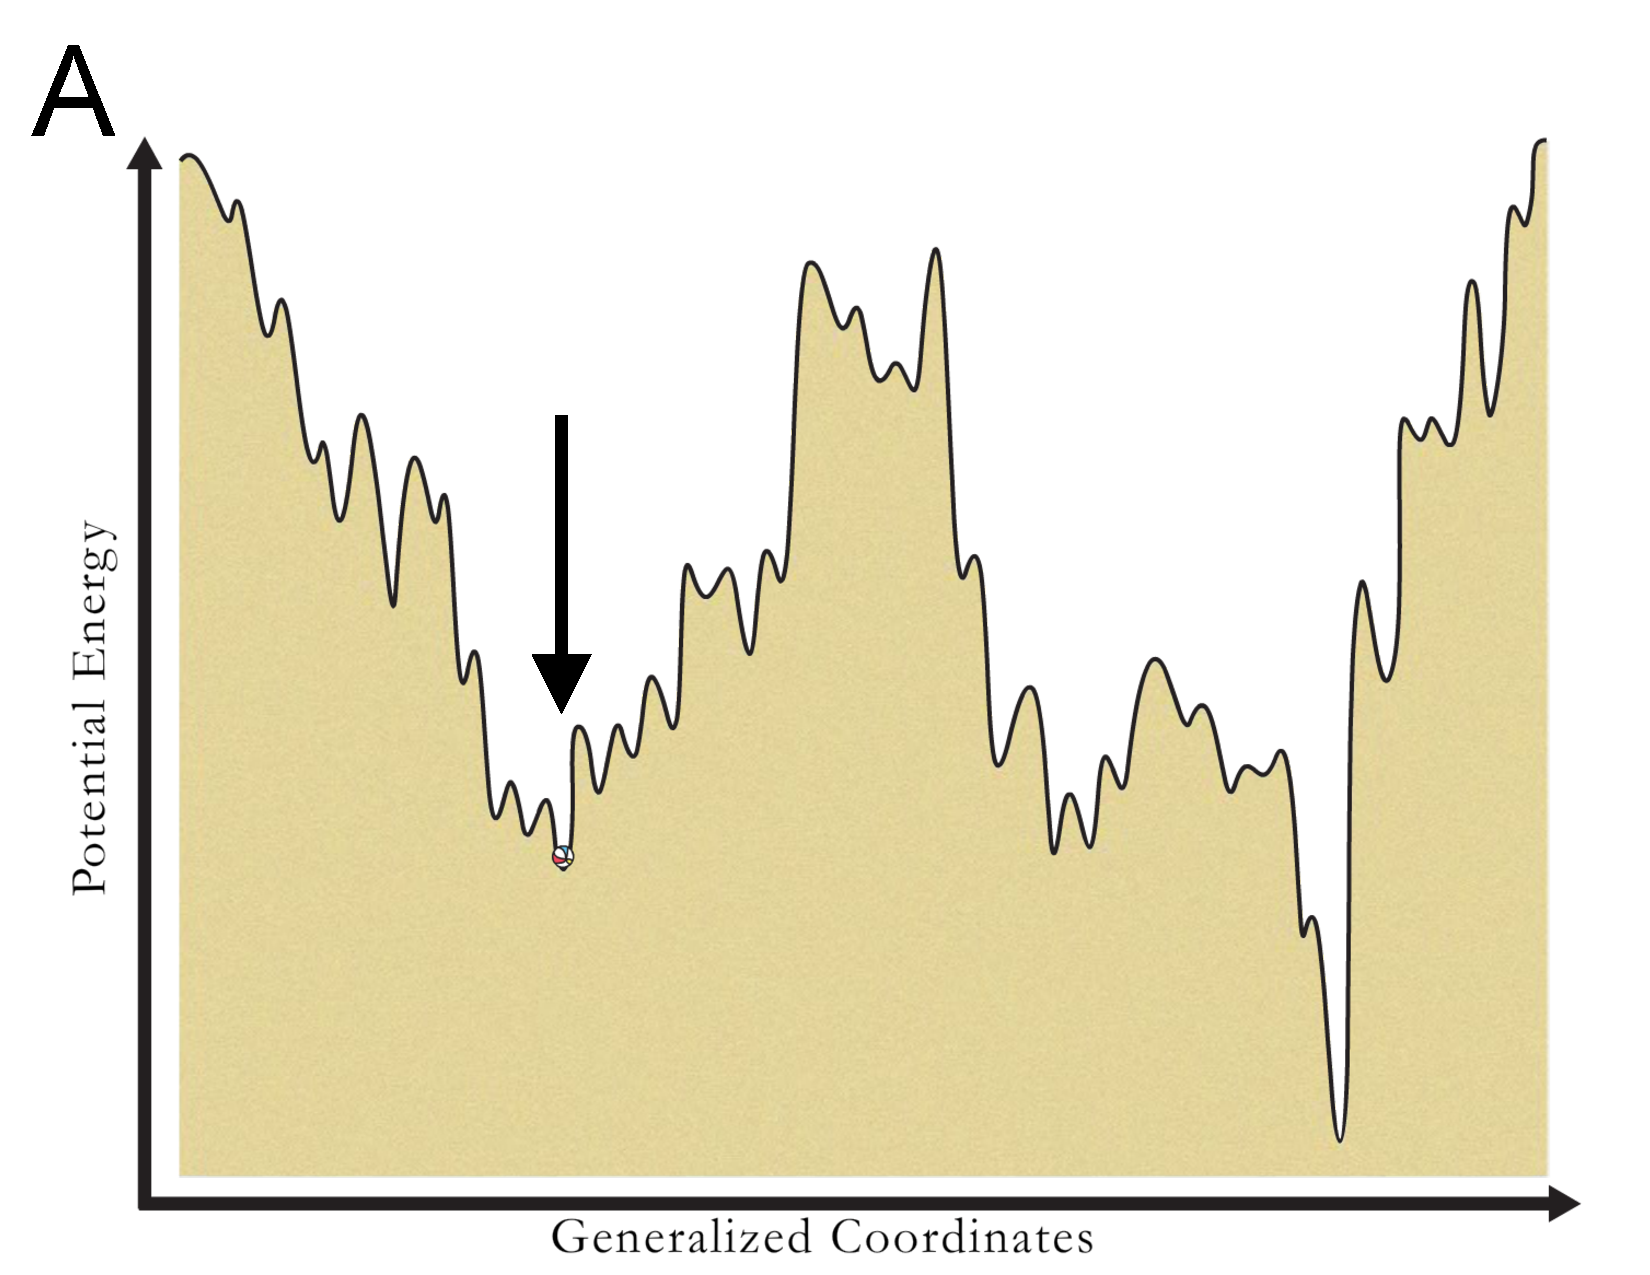
\includegraphics[width = .45\textwidth]{./Figures/MTD/MTD_1.pdf}
	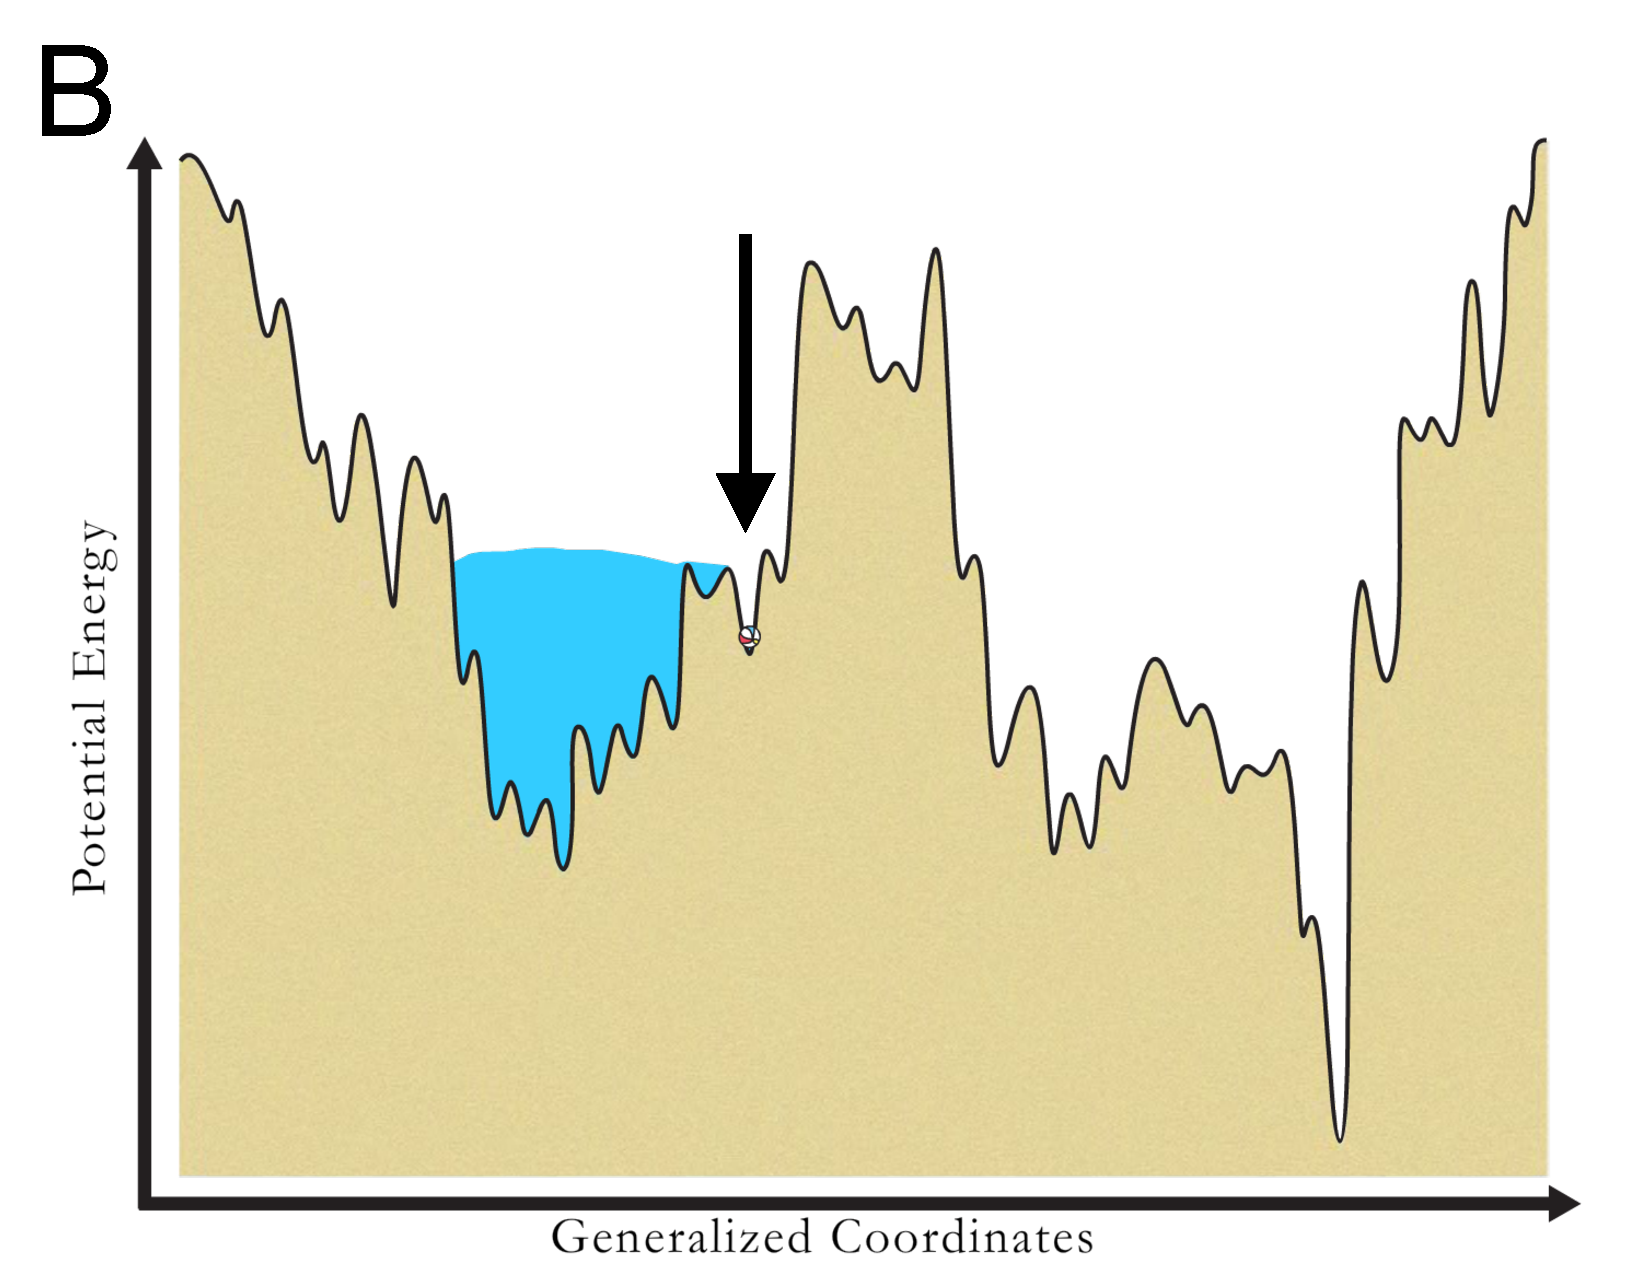
\includegraphics[width = .45\textwidth]{./Figures/MTD/MTD_2.pdf}
	\\
	\vspace{5mm}
	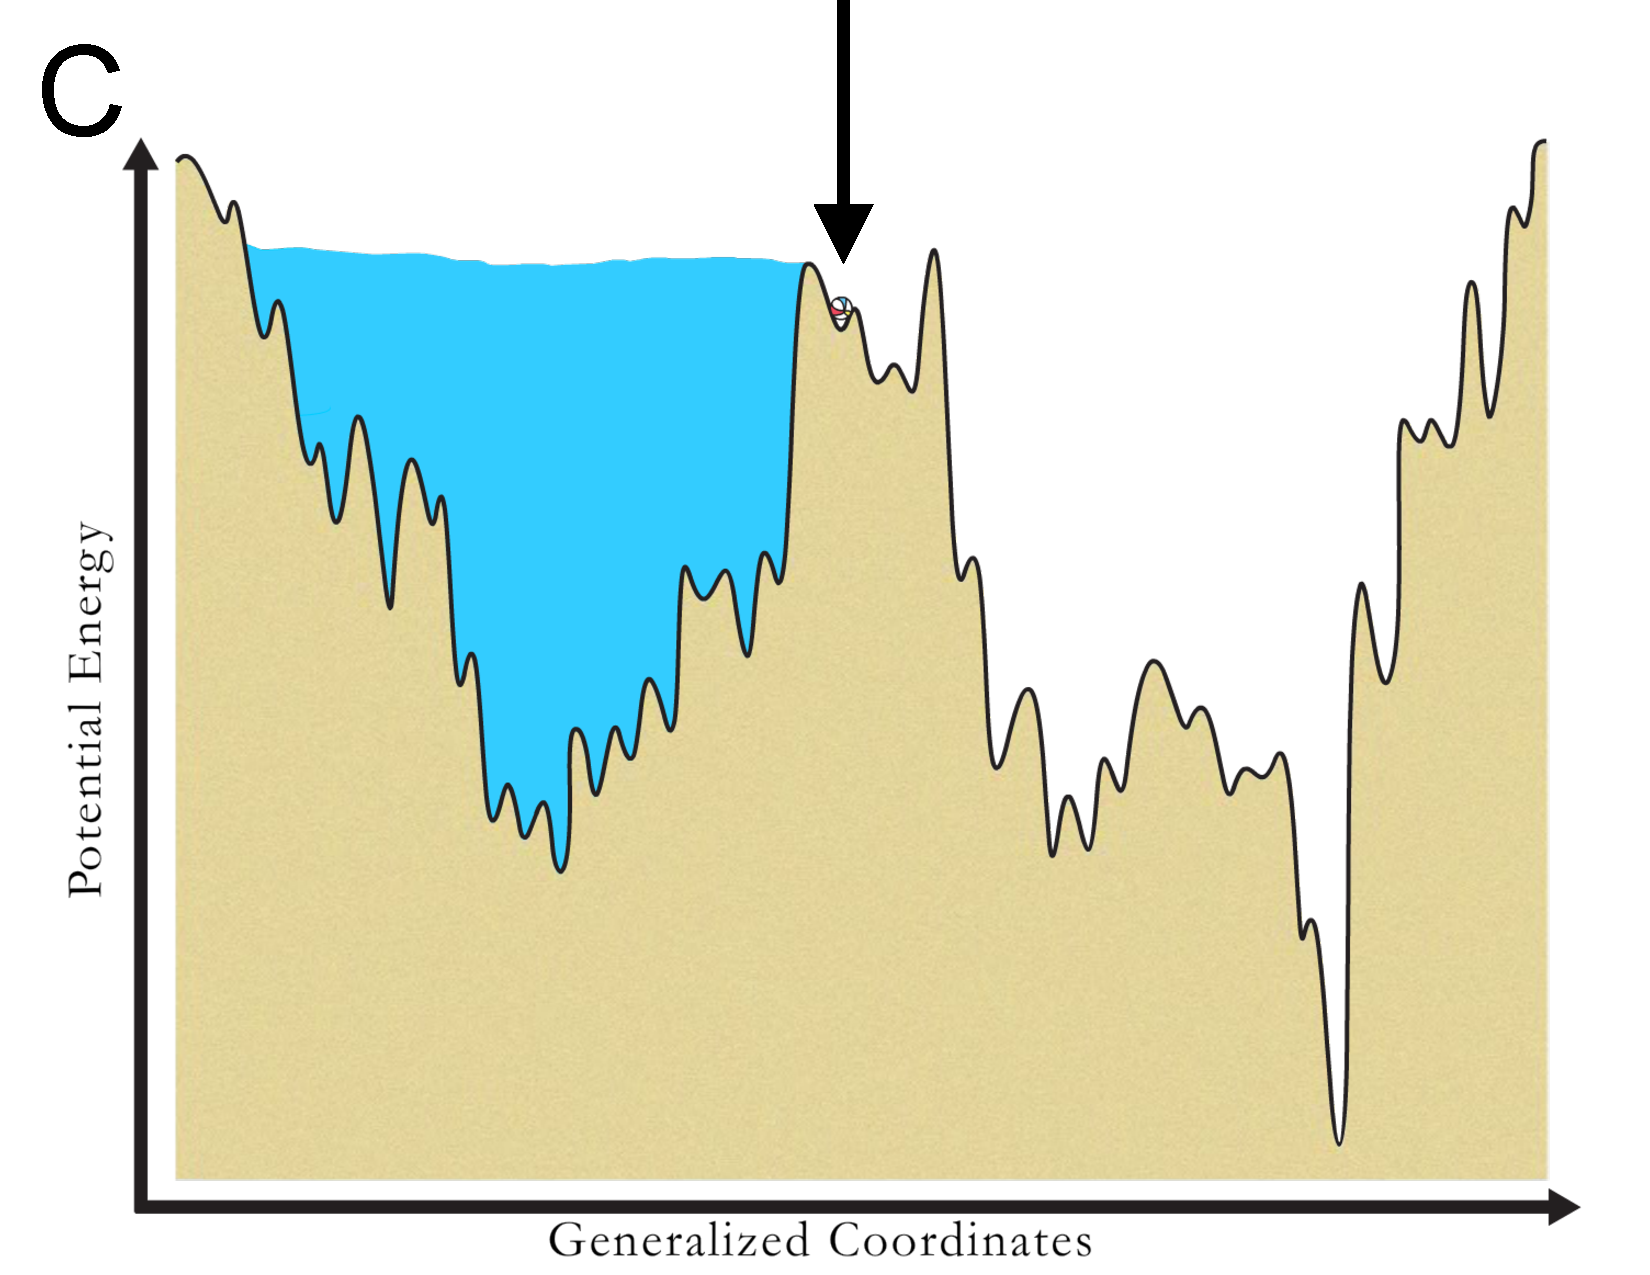
\includegraphics[width = .45\textwidth]{./Figures/MTD/MTD_3.pdf}
	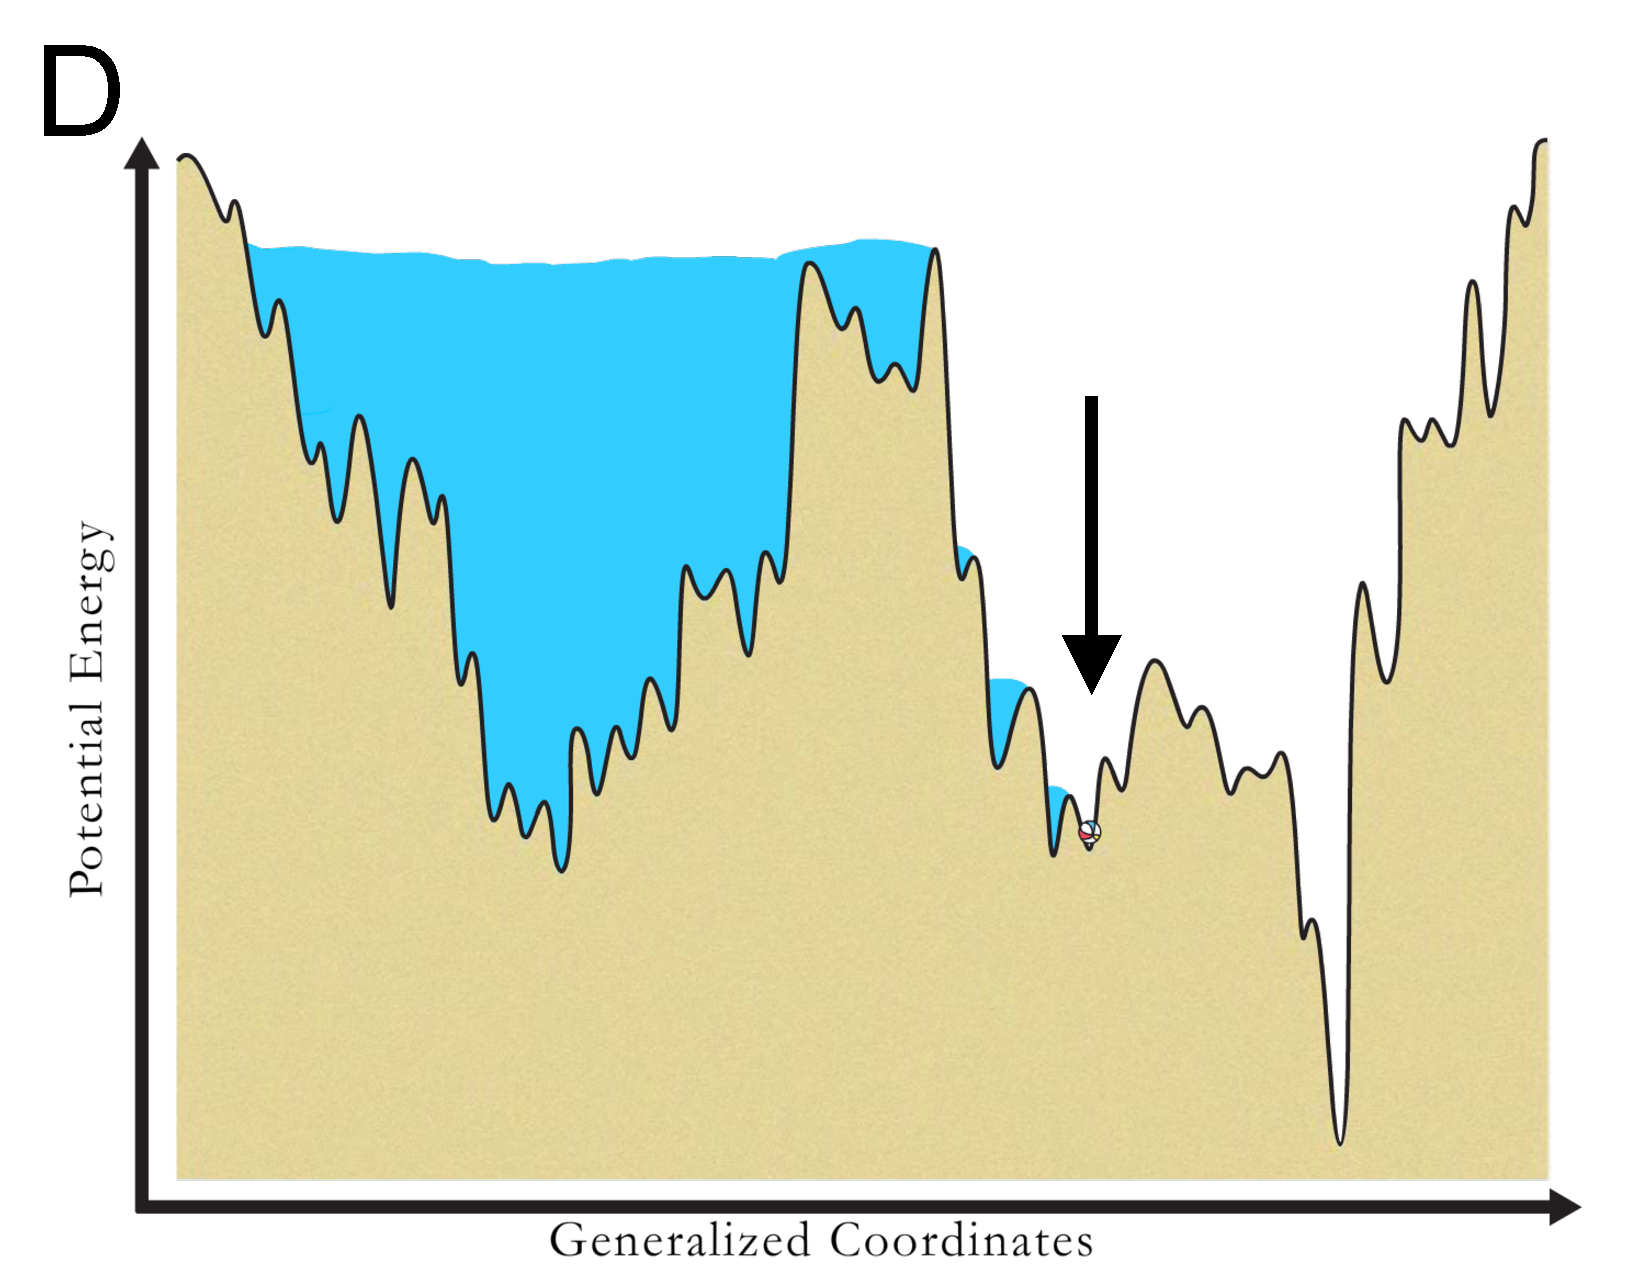
\includegraphics[width = .45\textwidth]{./Figures/MTD/MTD_4.pdf}
	\caption{These four figures depict the metadynamics method with application to the potential energy landscape framework.  The vertical axis is the potential energy of the system as a function of generalized coordinate.  The ball, pointed to by the arrow, indicts the current configuration of the system.  The tan region is inaccessible by the system.  Figure A shows the system starting in an energy minimum on the landscape.  From A to B, potential energy penalty functions are added in the form of Gaussians, shown in the figure by the blue region, which forces the system to evolve away from the original configuration and sample new energy minimums.  From B to C, application of many more penalty functions has resulted in the left side of the landscape filling allowing the system to now sample high energy configurations.  Lastly, from C to D, the system is driven over the large energy barrier separating two deep minimums allowing the system to now sample a very different area of the landscape, previously inaccessible in a molecular dynamics simulation.}
	\label{landscape filling}
\end{figure}

At this point, it is important to distinguish $\mathbf{r}_{\min}^\alpha$, which is a minimum on the $\Phi$-space potential energy landscape, and the $\mathbf{r}_{\min}$, which is a minimum on the inherent potential energy landscape $U(\mathbf{r})$ \cite{Kushima2009, Kushima2009a}.  These two minimums can be very different.  During a simulation, we sample far more minimums on the $\Phi$-space landscape, but it may require multiple penalties to overcome a barrier on the inherent landscape and sample a new minimum on the inherent landscape \cite{Kushima2009, Kushima2009a}.  Typically, $\phi(\mathbf{r},\mathbf{r}_{\min}^\alpha)$ is zero at a new minimum of the inherent landscape because as discussed above, the penalty functions are heavily localized.  The metadynamics simulation tracks the potential energy of the system as the system is biased over the landscape \cite{Kushima2009, Kushima2009a}.  Because the potential energy trajectory is known post computation, the minimums (basins) and saddles (barriers) can be calculated from this trajectory. 

\section{Implementation and Benchmarking}
The metadynamics method described above was implemented into the open-source molecular dynamics package GROMACS \cite{GROMACS}.  Details on the code's implementation and structure are discussed in Appendix \ref{code}.  Briefly, the method was implemented into the code such that the implementation does not affect GROMACS' other capabilities, thus the package is still a fully functional edition.  The code was implemented with OpenMP support to help reduce computational loads \cite{OpenMP}.  The parallelization is performed mostly on loops over atoms.  One issue noticed with parallelization is that it causes the code to no longer create reproducible results.  If the code is run serially, the results are always consistent for the same inputs.  However, because metadynamics has summations over thousands to millions of small numbers once several penalties have been applied, the parallelization of these summations leads to finite precision errors.  As a result, the first tens of penalties applied are consistent for the same input values, but once hundreds and thousands of penalties are applied finite precision arithmetic results in different trajectories along the potential energy landscape.  This is unavoidable, but also, presents no error in the final results as the finite precision errors merely leads to sampling the landscape in a different direction.  Due to the high dimensional nature of the landscape, finite precision errors leads to sampling along a different path of the landscape, but we assume that as long as a sufficiently long trajectory is sampled, the trajectory is representative of the landscape as a whole.

While algorithmically metadynamics is simple, implementation is computationally intensive.  In order to perform metadynamics, first the code must compute the pair potential forces in the system after every step, which alone is the most computationally demanding portion of a molecular dynamics simulation.  Then, we add computation of the force on the system imposed by all the penalties added, which requires a loop over all atoms for every penalty function applied.  Thus, after $\alpha$ penalties, metadynamics adds $\mathcal{O}(N\alpha)$ computations per iteration of Newton's steepest descent, which can become expensive. The initial metadynamics simulations required a large amount of computer time, far more than we expected, so while debugging we did time diagnostics to possibly increase the computational speed.  As a result, we calculated the time spent per penalty applied, and, because the number of penalties grows during the simulation, we noticed a linear increase in computational time per penalty as more penalties are applied.

The increase in time is because each new penalty leads to an additional loop over all the atoms for every iteration of Newton's steepest descent.  This significant increase in computational cost per penalty motivated us to add OpenMP parallelization.  Further, this motivated us to seek other forms of computational speed up, because the success of metadynamics is dependent on applying as many penalties as possible in an efficient manner.  A larger portion of the computation is performing Newton's steepest descent, which is dependent on the search parameter, $\alpha$.  $\alpha$ can be defined by the user, or several methods to compute the most efficient search parameter, $\alpha$, exists as well.  However, these methods require the calculation of the inverse of the Hessian matrix, which is extremely expensive of a computation for large matrices.  These methods are beneficial for small linear systems, but typical metadynamics systems have Hessian matrices of size $N\times N$ (typically $N$ ranges from large hundred to thousands), which is too expensive to compute. On the other hand, user fixed values can often be unstable or inefficient.  Thus, we decided that a dynamically determined search parameter is the optimal method.  Initially, the search parameter is set to an user estimated value. If Newton's steepest descent yields a step towards a minimum (energy was decreased), then the search parameter is increased by $20\%$.  If the search yields an increase in energy, then we reject the configuration and decrease the search parameter by $50\%$.  This resulted in significant speed-up from the fixed user value method.  Further, this provided another check for convergence of the algorithm.  We implemented that the Newton's steepest descent was converged if, either, a successful step resulted a percent change of potential energy less than an user defined threshold percentage, or an unsuccessful step resulted in a minimization search parameter less than 10e$-$5 nm.  While debugging, we noticed that the method typically converged by the energy criteria rather than the minimization step criteria.  

\begin{figure}[h]
	\centering
	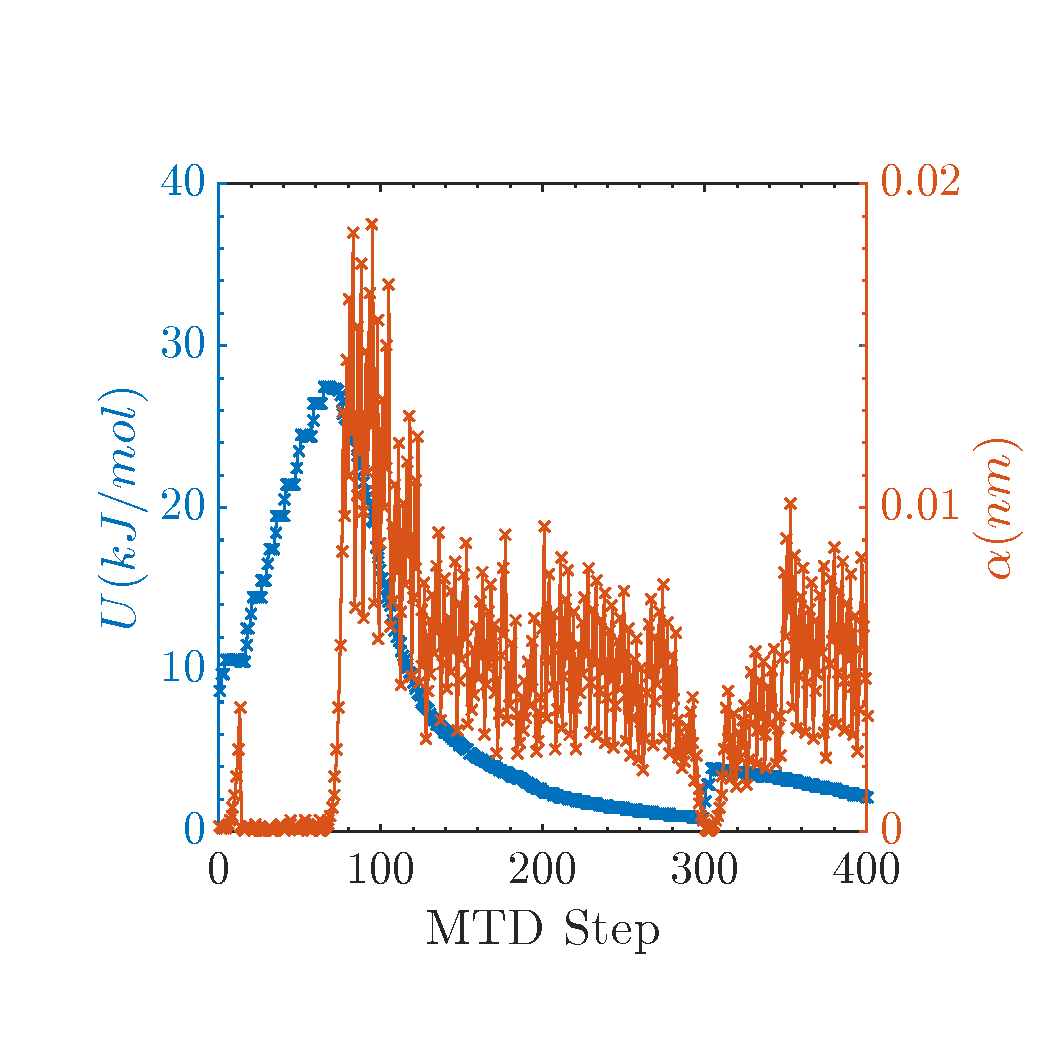
\includegraphics[width=.5\textwidth]{./Figures/MTD/dynamic_stepsize.pdf}
	\caption{Added penalty energy and minimization step size, $\alpha$, as a function of metadynamics iteration.  This figure shows the change in the added potential energy and minimization step size during convergence of one Newton's steepest descent.  The figure shows that as the energy is decreased the minimization step is dynamically increased and decreased.}
	\label{dynamic_stepsize}
\end{figure}

Figure \ref{dynamic_stepsize} shows the results once the dynamically determined search parameter was implemented.  The Figure shows the Newton's steepest descent for one convergence of a penalty function.  The figure shows that, at the start, the search parameter is small and, as successful steps are made, the search parameter increases as the potential energy is decreased.  Then, once the step size has become large, the steepest descent iteration results in an increase of energy (loss of stability), so the step size is decreased to retain stability.  Clearly, from this figure, the original value is significantly smaller than the average value used for $\alpha$, thus, showing the success of the method.  Note, this method resulted in a significant increase in computational speed with significantly less overhead than typical methods of determining $\alpha$, such as using the inverse of the Hessian matrix.

As explained in the previous section, the configurational coordinates used in our metadynamics method is the spatial coordinate of all atoms in the system, resulting in 3N degrees of freedom, where N is the number of atoms.   We first implemented this as the configurational coordinates of choice, and performed a simulation of a binary Lennard Jones system.  The simulation showed that after each penalty is applied, newton's steepest descent always resulted in the full minimization of the penalty energy.  This was universal across penalty heights and widths.  Once we visualized the simulation, the system was shown to have no internal relaxation of the atoms, instead the entire system drifted spatially.  From this, we learned that 3N degrees of freedom allows the system to minimize by drifting rather than internal reorganization.  Then, we removed the net force of the system, or removed three degrees of freedom.  As a result the force calculation for the metadynamics simulation becomes
\begin{equation}
	\mathbf{F}_i = \mathbf{F}_i - m_i\mathbf{A}
\end{equation}
where $\mathbf{A}$ is a three dimensional vector defined as
\begin{equation}
	\mathbf{A} = \frac{1}{N}\sum_{i}^N\frac{\mathbf{F}_i}{m_i}
\end{equation}
where $m_i$ is the mass of atom $i$ and $\mathbf{F}_i$ is the force vector of atom $i$.  By removing this net force from the system, the system internally reorganized to minimize the penalty energy, as we should expect.  Thus, our metadynamics method, and resulting landscape configurational coordinates space, has 3N-3 degrees of freedom.  

\section{Appropriate Simulation Parameters}
The metadynamics method has several user definable parameters (energy convergence percent change, initial energy minimization step size $\alpha$, maximum number of minimization steps, penalty function height H, penalty function width $\sigma$, and maximum penalties).  Most of these options have little impact on the computation and can therefore be chosen with ease.  Percent change for energy convergence affects the margin of error of the minimums sampled.  Initial energy minimization, step size can virtually be any number since the dynamic step size algorithm will correct for poor initial values, but generally a value on the scale of picometers is appropriate.  The maximum number of minimization steps can be on the order of a few thousand, as can the maximum number of penalties.  However, the penalty function width and height heavily influence the computation of the potential energy landscape.  

The penalty function width and height impact both the results of the potential energy landscape sampled and the computational speeds of the simulation.  As discussed in the previous sections, the potential energy landscape is rich with large and small energy barriers.  The simplified picture of the potential energy landscape presented previously gives the illusion that a single path along the landscape exists.  Contrary to this, a system has a plethora of paths to escape an energy minimum, each unique.  The potential energy landscape contains more energy minimums and energy barriers separating these minimums than is calculable in any reasonable compute time.  However, depending on the penalty energy function used in the metadynamics method, different paths and barriers will be preferentially sampled.  

To study the height and width dependence of the potential energy penalty functions, we performed several simulations on the Kob-Andersen model (the parameters for this model are provided in Section \ref{kob_andersen}).  The penalty height was varied while maintaining a constant width squared of .1 nm$^2$, and the penalty width was varied while maintaining a penalty height of 1 kJ/mol.  The results are summarized in Figure \ref{coarsening}.  Both the height and the width affects the path along the potential energy landscape taken by the metadynamics method, as shown in Figure \ref{coarsening}.  

\begin{figure}[h]
	\centering
	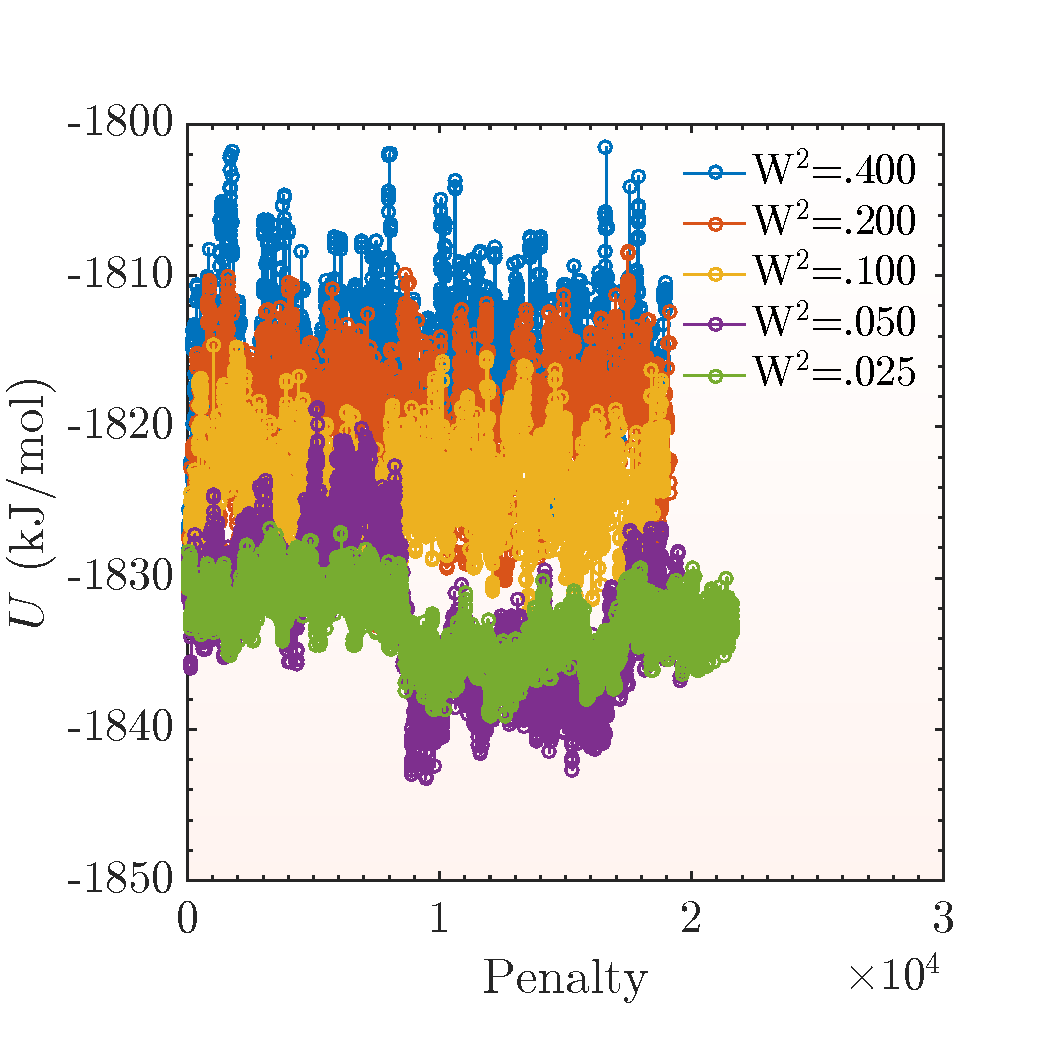
\includegraphics[width = .45\textwidth]{./Figures/MTD/width_dependence.pdf}
	\hspace{.01\textwidth}
	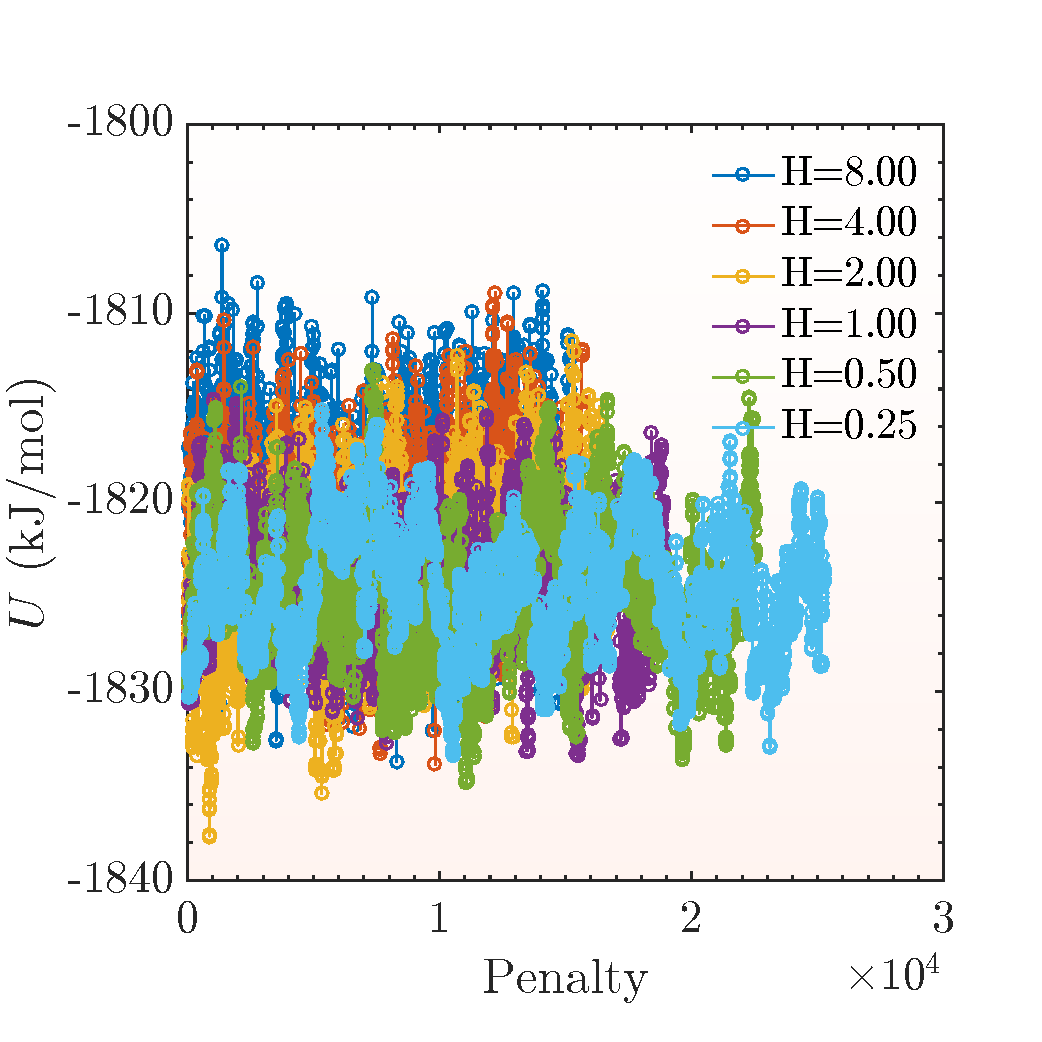
\includegraphics[width = .45\textwidth]{./Figures/MTD/height_dependence.pdf}
	\caption{Potential energy versus penalty number for various penalty function heights and widths.  The left figure shows the sampled potential energy landscape for varying penalty widths squared.  The right figure shows the sampled potential energy landscape for varying the penalty heights. For the width variation, the height of the barrier was fixed to 1 kJ/mol.  For the height variation, the width squared was fixed to .1 nm$^2$.}
	\label{coarsening}
\end{figure}

Figure \ref{coarsening} shows the effect of the two penalty function parameters, the height and width of the penalty.  The left figure shows the width dependence, and the right figure shows the height dependence.  The width should in theory affect how well a single penalty fills the energy basin currently occupied by the system.  If the width is too small, the penalty will under fill the broadness of the basin, and the system will inefficiently be biased out of the basin.  However, a penalty with a small width will provide high resolution landscape sampling.  The simulation will sample the small energy barriers of the landscape effectively, but will inefficiently sample the large barriers.  On the other hand, if the width is too large, the penalty will no longer obey the locality requirement of the penalty function.  The penalty function will affect the system in nearby basins as well as the current basin.  A large width will result in a penalty filling multiple basins.  As a result, the simulation provides a sampled landscape with poor resolution but efficiently samples large barriers.  From the figure, the small widths leads to a landscape sampled with low energy, with many low energy barriers sampled.  The simulation also leads to more penalties being applied.  The large widths resulted in much higher potential energy landscape sampling.  Thus, we can conclude that wide penalties leads to a more effective filling of basins.  A good estimate of an approximate width is from the approximate cage size of the system.  The cage size can be estimated from the mean squared displacement of the system, $\left<(r^2(t))\right>$, and the cage is where the ballistic regime ends.  For this system, this approximates to $\left<(r^2(t))\right> = 0.1$ nm$^2$, which from the figure we can see leads to a landscape that appears to not under fill the basins like the lower widths.  

Figure \ref{coarsening} also shows the height dependence of the penalty function.  The height affects how accurately the potential energy landscape is sampled.  If the height is small, the estimated values of the potential energy landscape will be very accurate, because the error of the values on the landscape are accurate to within the height of the penalty.  However, with a small height the basins are filled slowly, thus requiring vastly more penalties to overcome energy barriers.  This leads to a reduced sampling of the landscape.  If the height is large, the accuracy of the simulation is low, but the barriers are sampled very efficiently.  Thus there is an accuracy-efficiency trade-off for the height.  We see this in Figure \ref{coarsening}.  The small heights lead to more penalties applied, because small penalties are easier for steepest descent to converge on, however, less barriers are sampled overall.  On the other hand, the figure shows the largest penalty leads to low accuracy and sampling of only large barriers in the landscape.  Overall, the best estimation for a strong height is to use the pair potential's value for $\epsilon$, which is 1 kJ/mol for this system.  This is a good estimate, because $\epsilon$ is the depth of the basin on the two atom potential energy landscape for Lennard-Jones.  For non Lennard-Jones systems, the minimum value of the pair potential is the best estimate for the penalty height.  This value will sample the potential energy landscape efficiently while minimizing the error induced by larger penalty function heights.  Overall, the choice of the width and height is dependent on the desired resolution and efficiency desired.  If high resolution is desired, small widths and heights are needed.  If sampling a large portion of the landscape is desired, then large widths and heights are needed, but at the cost of resolution of the landscape.

\section{Mapping the Landscape to Temperature}
One aspect about metadynamics that has been overlooked is the concept of temperature.  Metadynamics simulations are performed without a temperature component, because the goal of the simulation is to sample the potential energy landscape.  Thus, in order to compare the simulation to experimental or MD results, the metadynamics results must be mapped to temperature in some manner.  The method to determine the mapping from temperature to potential energy is as follows \cite{Kushima2009, Kushima2009a}.  At various temperatures and the same density as the metadynamics simulation, molecular dynamics simulations are performed.  After set time intervals, $\Delta t$, the current configuration of the MD simulation is used as the initial configuration for energy minimization \cite{Kushima2009, Kushima2009a}.  The potential energy of the system after energy minimization is recorded, and then the MD simulation is continued from where it was prior to energy minimization.  This method was also employed by a research group to sample the potential energy landscape \cite{quench}.  The issue with this method for that purpose is that, like MC simulations, the energy barriers are not determined and there is no guarantee that subsequently sampled basins are adjacent on the landscape.  Also for temperatures near $T_g$, the system struggles to escape deep minimums, thus the method provides an unrepresentative sample of the potential energy landscape.  However, this method still serves as a method to map the inherent energy to the temperature. An example results of this method are shown in Figure \ref{temperature_cuts}. 

\begin{figure}[h]
	\centering
	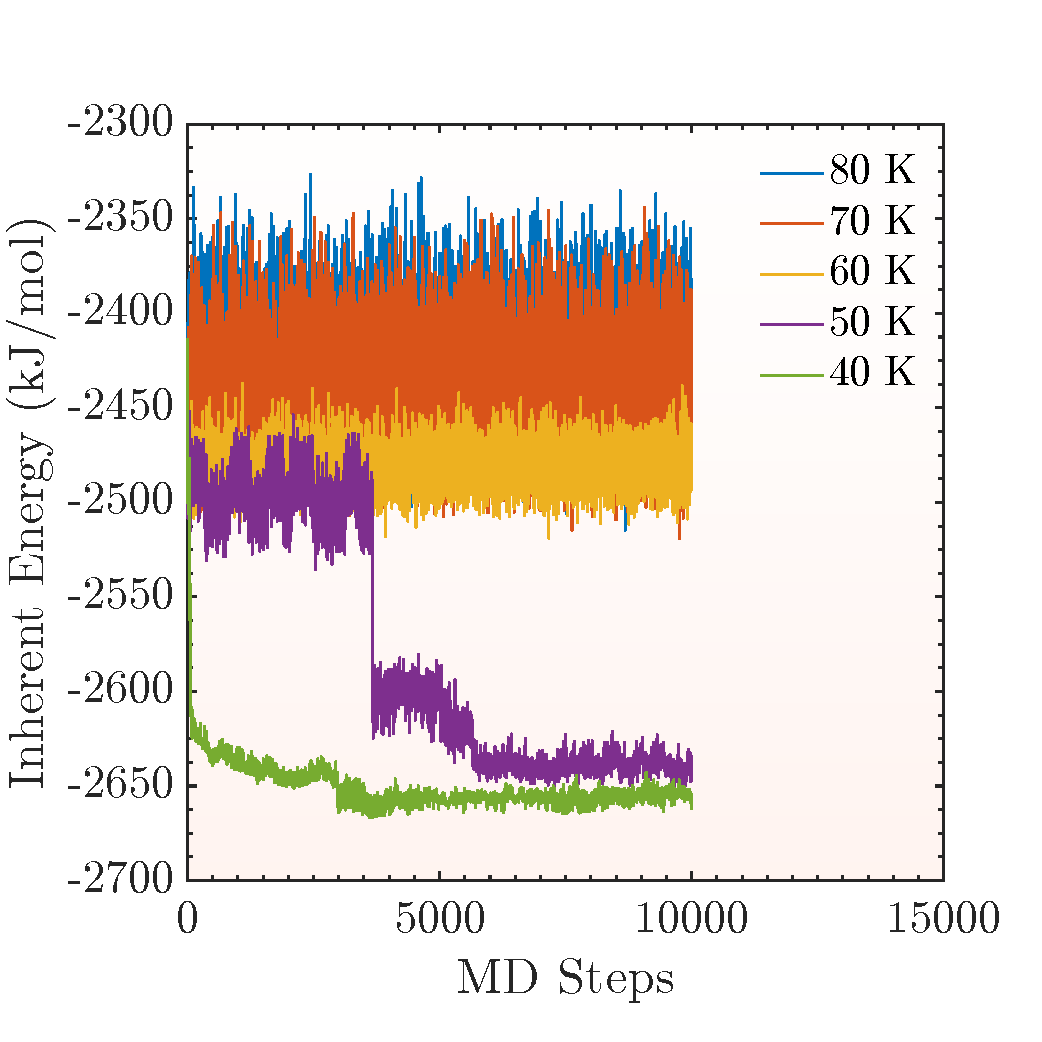
\includegraphics[width = .5\textwidth]{./Figures/MTD/temperature_cuts.pdf}
	\caption{Inherent energy plotted as a function of MD steps for various temperatures.  This figure shows the sampled inherent energies for calculating the mapping from inherent energy to temperature.  Clearly, there is a transitional temperature around 50 K to 60 K.  Below this temperature the sample values are concentrated around a particular value, and above this temperature the sample values have a large standard deviation.}
	\label{temperature_cuts}
\end{figure}

Figure \ref{temperature_cuts} shows the potential energy determined by energy minimization periodically during an MD simulation.  As the figure shows, at high temperatures, the simulation samples a wide range of energy values because at high temperature, the system has the thermal energy to overcome high energy barriers and freely sample the entire landscape.  As the temperature is decreased, the landscape begins to dominate the dynamics, and the energies sampled begin to decrease in value and in variance, until only discrete values are sampled.  If sufficiently large numbers of samples are taken along the MD simulation, we can plot the average inherent energy versus temperature, shown in Figure \ref{sample_mapping} \cite{Kushima2009, Kushima2009a}.

\begin{figure}[h]
	\centering
	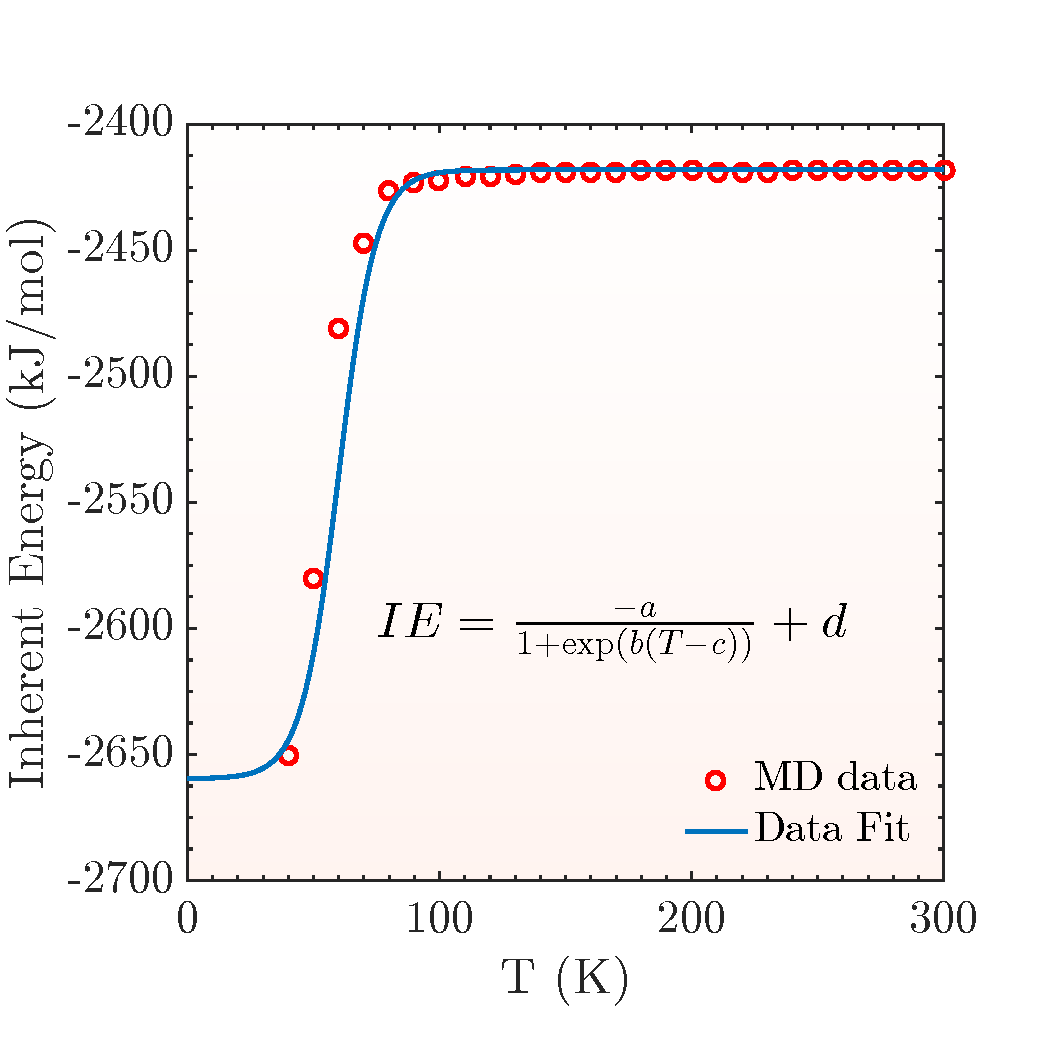
\includegraphics[width = .5\textwidth]{./Figures/MTD/example_mapping.pdf}
	\caption{Inherent energy plotted as a function of temperature.  This figure shows the data values determined from MD simulations in red open circles, and the data fit used to determine the mapping from inherent energy to temperature as a solid blue line.  The figure shows the equation used to fit the data. }
	\label{sample_mapping}
\end{figure}

Figure \ref{sample_mapping} shows the average inherent energy (IE) as a function of temperature (T), the red circles show the values computed by the MD simulations.  This figure shows that at high temperatures higher inherent energies may be sampled by the system.  In order to create a relationship between the inherent energy and the temperature, the MD data is fit with a line.  The MD data is fit to the line with the following equation
\begin{equation}
IE = \frac{-a}{1+\exp\left(b\left(T-c\right)\right)} + d
\end{equation}
where $IE$ is the inherent energy of the system, $T$ is the temperature in Kelvin, and $a$ is a fitting parameter calculated as $a=\max\left(IE\right) - \min\left(IE\right)$, $b$ is a free fitting parameter calculated by Matlab to best fit the data, $c$ is a fitting parameter calculated as the temperature value located at $\frac{a}{2}$, and $d$ is a fitting parameter calculated as $d=\max\left(IE\right)$.  This equation form was chosen because the shape of the data is assumed to be a logistic function.  At high temperatures, the system will sample a large range of configurations with a large range of inherent energies.  At temperatures below, but near the melting temperature, the system will no longer have the thermal energy to sample high inherent energy configurations with high frequency.  The frequency with which inherent energies are sampled will decay exponentially, until a cross over temperature is reached.  Below this temperature, the system will get stuck in local minimums and not have the thermal energy to escape, leading to sampling of only low inherent energy values.  Thus, we assume a constant value at high temperature, a constant value at low temperature, and a logistic regression over all temperature.

\section{Measure of Atomic Structure}
\label{bop_calculation}
To study phase transitions, we need to know the structural changes that occur in the system during the simulation.  Many different order parameters exist to measure atomic structure, for example, the structure factor, the pair distribution function, or Voronoi polygons, to name a few.  While each of these order parameters have use and merit in certain situations, they do not fully capture the information we seek in identifying a nucleation site.  

Liquid to solid phase transitions are characterized by unique structural changes.  The liquid state is isotropic (independent of direction) while the crystal state is anisotropic experiencing order in preferential crystallographic directions.  The crystal state has both translational and rotational order, which does not exist in the liquid.  Further, the crystal state shows long range repetition of atom positions in certain crystallographic directions.  Typical measures of atomic structure such as the static structure factor or pair distribution function are useful for showing the difference in the structure between the liquid state and crystal state.  However, they are sensitive to the orientation of the crystal structure.  Further, while many studies have used the first peak in the structure factor to measure the structure during a phase transition, the parameter fails to provide local information of the structure.  The structure factor and pair distribution function are system averaged quantities that do not provide information about where areas of high and low structure exists during the phase transition.  This makes these parameters unsuitable for studying the structure of the system during nucleation.

As the name implies, one such order parameter that is orientationally invariant and provides information on the local degree of structure on a per atom basis is the local bond orientational order parameter (BOP).  The local bond orientational order parameter is a quantity for measuring medium and short range order in a system.
$q_l$ is the bond order parameter for individual atoms in the system, $Q_l$ is the system wide bond order parameter, $l$ is the order of the bond order parameter (typical values are 4 and 6), $i$ is the atom number, $t$ is the time. $Q_l$ is equivalent to $q_l$ averaged over all the atoms in the system \cite{BOP_first}. $\bar{q}_l$ is equivalent to $q_l$ averaged over an atom's nearest neighbors, this has the benefit of reducing the overlap of liquid and crystal values \cite{BOP}. This quantity cannot be compared to experiments but can be very useful for determining structural order and phases in a system. The quantities are defined as below. The bond order parameter per atom is defined as
\begin{equation}
q_l(i,t) = \sqrt{\frac{4\pi}{2l+1} \sum_{m=-l}^l\left|q_{lm}(i,t)^2\right|}
\end{equation}
where
\begin{equation}
q_{lm}(i,t) = \frac{1}{N(i)}\sum_{j=1}^{N(i)}Y_{lm}(\hat{r}_{ij}(t))
\end{equation}
$m$ ranges from $-l$ to $l$, $N(i)$ is the number of nearest neighbors around atom $i$, and $Y_{lm}$ is the spherical harmonic of order $l$ and $m$, and $\hat{r}_{ij}$ is the unit vector between atom $i$ and $j$. The unit vector can be converted to spherical coordinates which are required for the spherical harmonics. The full system bond order parameter of the system is defined as
\begin{equation}
Q_l(t) = \sqrt{\frac{4\pi}{2l+1} \sum_{m=-l}^l\left|Q_{lm}(t)^2\right|}
\end{equation}
where 
\begin{equation}
Q_{lm}(t) = \frac{\sum_{i=1}^NN(i)q_{lm}(i,t)}{\sum_{i=1}^NN(i)}
\end{equation}
and $N$ is the number of atoms in the system. The nearest neighbor averaged bond order parameter is defined as
\begin{equation}
\bar{q}_l(i,t) = \sqrt{\frac{4\pi}{2l+1} \sum_{m=-l}^l\left|\bar{q}_{lm}(i,t)^2\right|}
\end{equation}
where
\begin{equation}
\bar{q}_{lm}(i,t) = \frac{1}{N(i)}\sum_{j=0}^{N(i)}q_{lm}(j,t)
\end{equation}
Lastly,
\begin{equation}
\bar{Q}_l(t) = Q_l(t)
\end{equation}
there is no difference between the system bond order parameter and the nearest neighbor averaged system bond order parameter.  The nearest neighbors are defined as the atoms within a cutoff distance of a particular atom.  The cutoff distance is typically determined to be the distance of the first peak of the pair distribution function.  Using a smaller value leads to smaller bond orientational order parameter values.

\begin{table}
	\centering
	\caption[Mean values for the bond orientational order parameters for several crystal structures for a monoatomic Lennard-Jones liquid.]{Mean values for the bond orientational order parameters for several crystal structures for a monoatomic Lennard-Jones liquid \cite{BOP_first,BOP_values}.}
	\label{BOP_values}
	\begin{tabular}{ c c c c c c c c }
		& $Q_4$ & $Q_6$ & $q_4$ & $\bar{q}_4$ & $q_6$ & $\bar{q}_6$ \\
		\hline	
		\hline		
		BCC & .0820 & .5008 & .0899 & .0334 & .4405 & .4080\\
		FCC & .1909 & .5745 & .1709 & .1582 & .5073 & .4914\\
		HCP & .0972 & .4848 & .1079 & .0841 & .4454 & .4218\\
		liq & .0000 & .0000 & .1090 & .0312 & .3601 & .1620\\
		\hline 
	\end{tabular}
\end{table}

